\section{Illistrative Examples of Tracking Resource Usage}
\label{sec:example}

We illustrate our technique for static checking of dynamic resources
through two example applications.  First is the surge application in
SOS that uses dynamiclly allocated memory to pass data buffers through
protocol stacks.  Second is the generic base component from TinyOS
that uses swapping of staticlly allocated messages to efficently
implement an interface to receive data messages.  Running on hardware
without memory protection, improper management of either the SOS
buffers or the TinyOS messages can lead to corruption of data or
simply crash the sensor node.

%
% NOTE (ROY): I am not sure that the following figure is doing
% anything other than taking up space.  I will remove it for now.
% 10-18-06
%
%\begin{figure}[t]
%\centering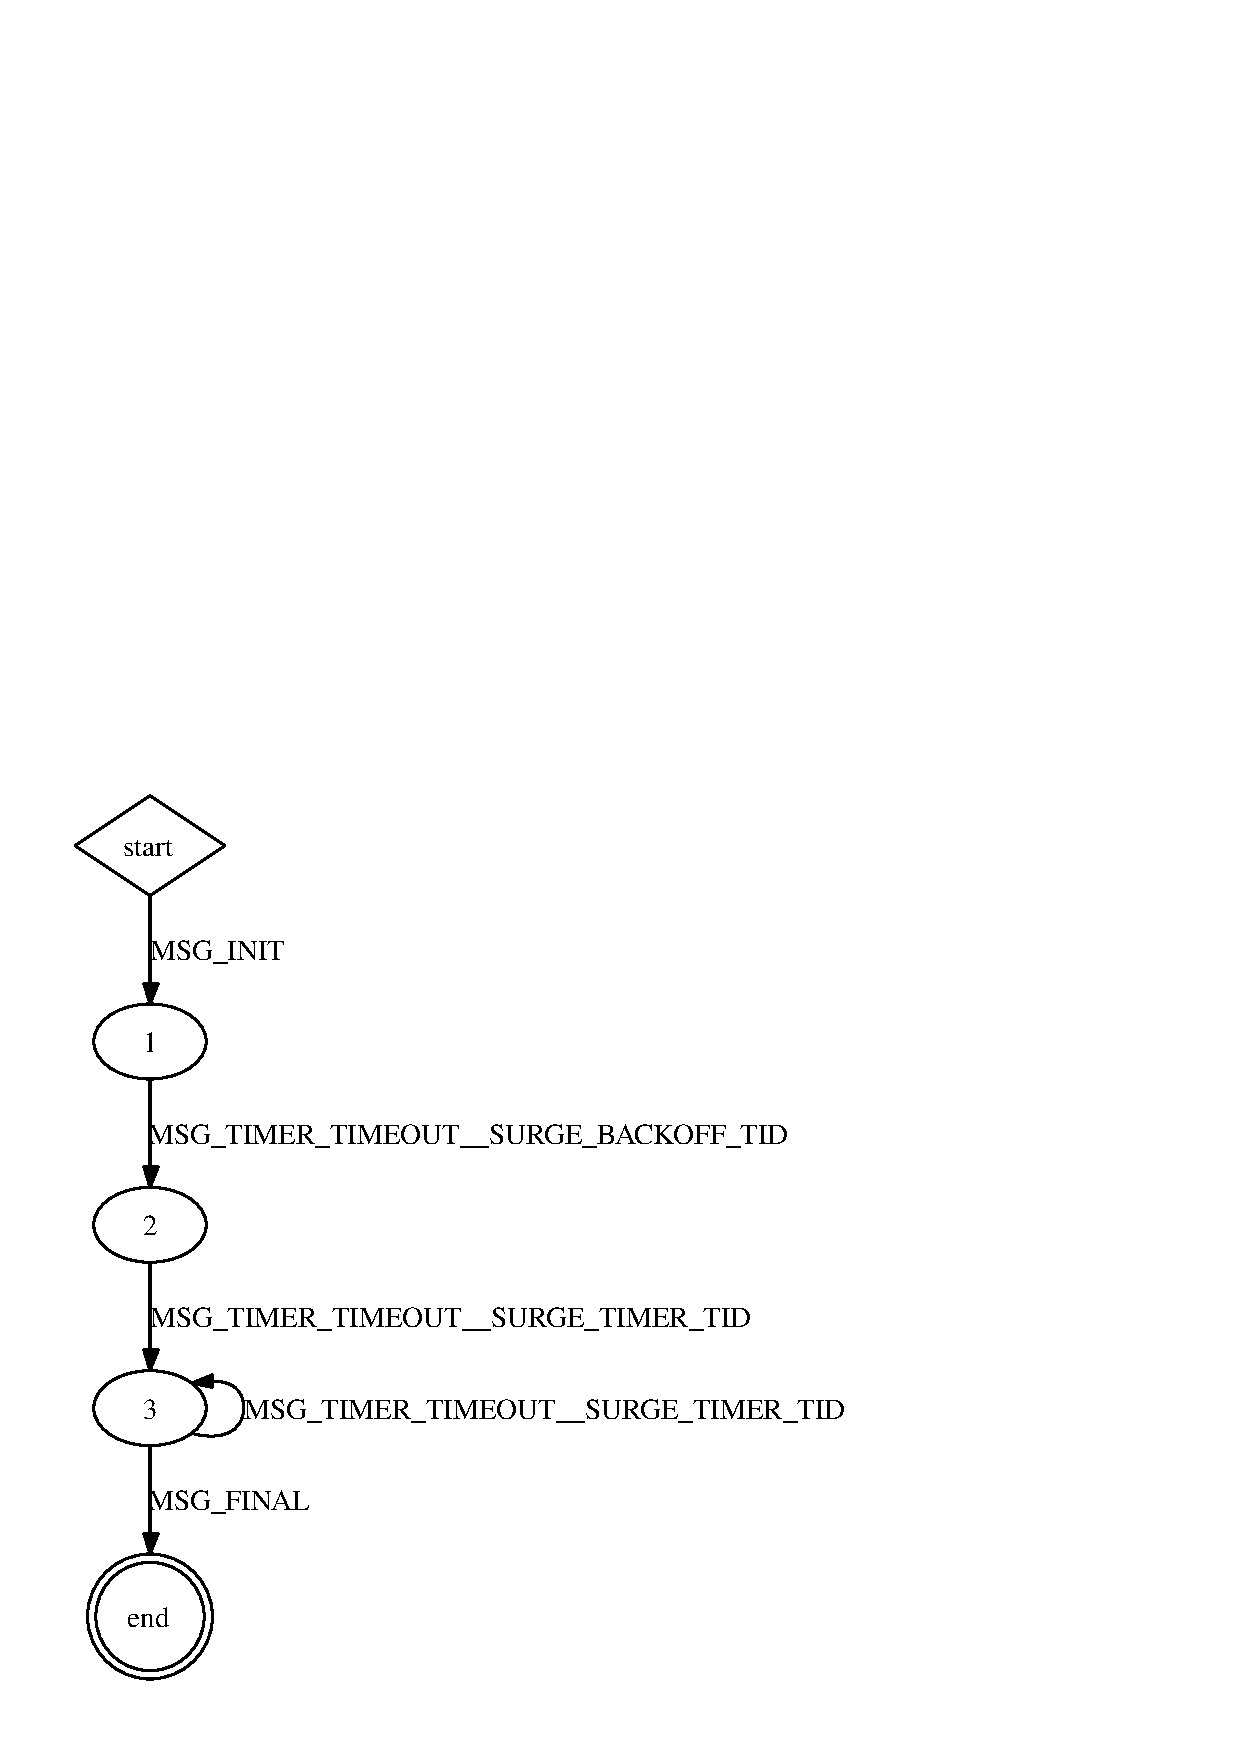
\includegraphics[angle=270,width=4.1in]{surge}
%\caption{{\tt surge} dataflow\label{fig:surge-dataflow}}
%\end{figure}


\subsection{Resource useage in {\tt surge}}

\begin{figure}[t]
\input{surge.c}
\caption{SOS implementation of {\tt surge}\label{fig:surge}}
\end{figure}

Figure~\ref{fig:surge} shows a portion of the SOS module that
implements {\tt surge}, a simple sensor network application that takes
sensor readings and sends the readings over a multihop network to a
base station~\cite{nesC}.  The function {\tt surge\_module} is the
entry point into {\tt surge} for messages from the kernel and from
other modules.  The function takes two arguments: a pointer to the
module's persistent state, which is saved in the kernel, and a pointer
to the current message.  A {\tt switch} statement is used to direct
each message type to an appropriate handler.  The handlers of interest
in this example are for the messages types {\tt MSG\_DATA\_READY} and
{\tt MSG\_TR\_DATA\_PKT}.

A sensor sends the message {\tt MSG\_DATA\_READY} to the surge module
when requested sensor data is ready to be read. The sensor data is
passed as the {\tt data} field of the message, which in general always
contains a message's payload.  Upon receiving this message, the {\tt
surge} message handler allocates a new packet ({\tt ker\_malloc}) to
be sent to the base station and posts a message ({\tt post\_long}) to
the tree-routing module in order to forward the sensor data.  The {\tt
post\_long} call is asynchronous, causing the kernel to package up all
the given arguments into a {\tt Message} structure and to schedule
this message for eventual delivery.

The message {\tt MSG\_TR\_DATA\_PKT} is sent by the tree-routing
module when data is received at the base station node.  Upon receiving
this message, the {\tt surge} message handler confirms that the
current node is the base station.  If so, the message handler forwards
the data to the UART driver via an asynchronous message send ({\tt
post\_net}).

The SOS kernel provides an API for programmers to manage dynamic
memory.  As shown in Figure~\ref{fig:surge}, the {\tt ker\_malloc}
function acts as expected, allocating a new block of memory.  The
kernel also provides a {\tt ker\_free} function for destroying
dynamically allocated memory.  Additionally, ownership of dynamic
memory can be transfered between modules through the messaging
interface provided in SOS.

%
% NOTE (ROY): This is not adding much to the discussion.  10-18-06
%
%In order to provide a simple form of automatic garbage collection for
%dynamically allocated memory, the SOS kernel imposes an {\em
%ownership} model on dynamic memory~\cite{sos}.  Each block of memory
%has a unique owner at any point in time, and the kernel maintains a
%mapping from each block of memory to its owner.  A block's initial
%owner is the module that allocates that block.  For example, the call
%to {\tt ker\_malloc} sets the {\tt surge} module as the initial owner
%of the newly allocated block.  When a module is removed from the
%system at run time, the kernel automatically frees all memory owned by
%that module.

Transfer of dynamic memory ownership occures at the end points of a
message.  First, the owner of a block of dynamically allocated memory
can explicitly {\em release} ownership of that block when it is passed
as the payload in a message.  This is accomplished by setting the
\texttt{SOS\_MSG\_RELEASE} flag in the corresponding {\tt post\_*}
call.  For example, the {\tt surge} module releases ownership of the
newly allocated {\tt pkt} upon sending it to the tree-routing module.
Second, a module can acquire ownership of a message's payload, which
is stored in the {\tt data} field, by calling
\texttt{ker\_msg\_take\_data} on an incoming message.  The function
returns a pointer to the message's payload.  For example, if the
current node is the base station, the {\tt surge} module explicitly
takes ownership of the given message's data under the name {\tt
payload}.

There are four release/take scenarios to consider.  If data is both
released by its sender and taken by its receiver, then ownership of
the data is transferred from the sender to the receiver.  If data is
released by its sender but not taken by its receiver, then the kernel
automatically frees the memory after the receiver's message handler
completes.  If data is not released by its sender but is taken by its
receiver, then the sender keeps ownership of the original message and
the receiver gains ownership of a new block of memory containing a
copy of that data.  Finally, if the data is not released by the sender
and not claimed by the receiver, then the sender keeps ownership of
the original message and the receiver has direct access to
``borrowed'' data for a limited period of time.  This last case is not
generally used in SOS due to the synchronization complications that
can result.


\subsection{Resource useage in {\tt GenericBaseM}}

\begin{figure}[t]
\input{surge.c}
\caption{TinyOS implementation of {\tt GenericBaseM recieve
interface}\label{fig:genericbase}}
\end{figure}


Figure~\ref{fig:genericbase} shows a portion of the TinyOS component
that implements the {\tt receive} event handler for {\tt GenericBaseM},
an application that uses a sensor node as a bridge between a base
station and the rest of a sensor network.  The {\tt receive} event
handler is passed in a {\tt TOS\_MsgPtr} pointing to the incoming
message and a flag describing where the message source.  If there are
no messages waiting to be sent, the handler forwards the message out
over the bridged interface and returns a pointer to a free message
buffer.  If a message is currently pending, the handler simply ignores
the message and returns the incoming message buffer to be reused.

A key property demonstrated by this TinyOS component is that of buffer
swapping.  Buffer swapping is throughout systems when dynamic buffer
creation is not desired or when dynamic buffer creation is simply not
allowed and is is a common technique used within TinyOS to allow data
to quickly pass through stacks of components.  Rather than
dynamicallyl allocating a new buffer, a call stack can simply return a
free buffer to the caller.  In the the TinyOS environment, handlers
that implement buffer swapping have implict memory ownership
responsibilities.  The handler can be though of needing to claim the
incoming {\tt TOS\_MsgPtr} and release a buffer to the caller.  Note
that this can be accomplished by returning the incoming buffer.


%%%%%%%%%%%%%%%%%%%%%%%%%%%%%%%%%%%%%%%%%%%%%%%%%%%%%%%%%%%%

\subsection{Static Ownership Checking}

SOS's original concept of ownership as described above provides
developers with a framework for designing modular programs. While this
can help reduce the complexity of managing dynamic memory, it is not
sufficient to prevent memory errors such as dangling pointers and
memory leaks.  For example, nothing prevents a module from freeing
some memory while another module (or even the same module) still has a
pointer to that memory.  If that pointer is ever accessed later, an
invalid dereference will result.  

A similar problem can occure with buffer swapping in TinyOS.  A TinyOS
component can improperly return a pointer to a buffer that is not yet
free during a buffer swap.  From that point on two components in the
system belive that they own the same buffer.  This leads to
unpredictable and unintional sharing of the buffer.

%
% NOTE: This depends on the garbage collection comment above
%
% Further, simple garbage collection introduces the potential for more
% dangling pointer errors, since the removal of a module implicitly
% frees the memory it owns, even if other modules have pointers to
% that memory.

In this work, we augment the often implicit ownership directives in
sensor network operating systems to provide a protocol governing
memory management that is sufficient to ensure the absence of memory
errors.  Our protocol makes explicit a common programming idiom in
sensor-network systems, whereby data is rarely shared but instead
follows a producer/consumer model.  We have built a tool that checks
for violations of this protocol on each SOS module at compile time.

Informally, the rules of the protocol can be stated as follows:
%
\begin{itemize}
%
\item A module may only manipulate the memory that it owns.
%
\item A module that takes ownership of a block of memory (either
through a function that allocates data or via a transfer of ownership)
must either free that memory, release it, or store it in the module's
persistent state.
%
\item A module may only free or release memory that it owns.  After a
module frees or releases memory, it may not access or update that
memory.
%
\end{itemize}
%
Because only the owner can manipulate or free its memory, dangling
pointers are avoided.  Because all memory must be either freed,
released or persistently stored by its owner, memory leaks are
avoided.


\subsubsection{Applying Ownership Protocol to {\tt surge}}

The {\tt surge} module described above can be showen to adhere to this
ownership protocol.  The {\tt MSG\_DATA\_RDY} message handler
allocates {\tt pkt} and takes ownership. This pointer is then
dereferenced in order to provide the sensor data to be sent up the
routing tree.  This pointer manipulation is safe since the module has
ownership.  The module then releases ownership by posting {\tt pkt} to
the tree routing module using the {\tt SOS\_MSG\_RELEASE} tag.  After
this release, the module does not access {\tt pkt} again and does not
store it, ensuring that access to the pointer is indeed released. 

The handler for {\tt MSG\_TR\_DATA\_PKT} also conforms to the
protocol.   When the current node is the base station, the handler
explicitly acquires ownership of the message's data using {\tt
ker\_msg\_take\_data}.  This allows the module to manipulate the data
and to pass it to the UART.  The {\tt post\_net} call explicitly
releases the data, fulfilling the module's obligation to that data.
After the release, the data is no longer accessed or stored.

While the {\tt surge} code is correct, small changes to the code can
easily cause problems to occur at run time, and our static checker
catches these potential errors.  For example, suppose the handler for
{\tt MSG\_DATA\_READY} did not release ownership of {\tt pkt} by
setting the {\tt SOS\_MSG\_RELEASE} flag in the call to {\tt
post\_long}.  In that case, the module would leak the memory allocated
for {\tt pkt}.  Indeed, our checker flags this modified version of the
code as erroneous, since {\tt surge} would not be freeing, releasing,
or storing the data for which it has taken ownership.


\subsubsection{Applying Ownership Protocol to {\tt GenericBaseM}}

It is also easy to show that the {\tt GenericBaseM} module follows the
ownership model described above.  Upon entry to the {\tt receive}
event handler the {\tt GenericBaseM} component owns the buffer
referenced by the global variable {\tt ourBuffer} and gains ownership
of the {\tt received} buffer passed into the function.  Within the
body of the function the handler, these are the only two buffers
accessed, although they are at times accessed via the alias {\tt
nextReceiveBuffer}.  At the end of the handler the buffer aliased by
{\tt nextReceiveBuffer} is returned to the calling function.  Note
that regardless of the path taken through the handler, at the call to
return the returned buffer is distinct from the buffer presistently
stored in {\tt ourBuffer}.  Thus the returned buffer is not accessed
by this component after the call to return.


\subsection{Function Attributes}

Our analysis is {\em modular}:  each function in a module or component
is analyzed in isolation.  To make checking of a function body precise
in the presence of calls to other functions, we employ {\em ownership
attributes} for function headers that capture the memory-related
behavior of a called function.  We add two attributes to the C code:
{\tt lh\_claim} and {\tt lh\_release}.  A formal parameter or return
value that has the {\tt lh\_claim} attribute indicates that the caller
must take ownership of the associated memory after a call.  This
annotation, for example, would be used to annotate a function that
wraps a call to {\tt ker\_malloc} within SOS, allowing that function's
callers to be properly checked without access to the function's
implementation.  Similarly, an {\tt lh\_release} attribute on a formal
parameter indicates that ownership of the parameter is transferred
from the caller of the function to the callee.  If a parameter does
not have an ownership attribute, memory ownership is unchanged.  Our
tool ensures that these attributes are employed wherever necessary,
when checking the implementation of each function.  In practice, we
have found that a small set of annotations is sufficient for precise
analysis.


